\documentclass[12pt]{article}
\usepackage{enumitem}
\usepackage{amssymb}
\usepackage{graphicx}
\author{Vincent Zheng}

\begin{document}

\title{CSE 215 - Homework 1}
\maketitle

\section*{Problem Set 1}
\begin{enumerate}[label = \alph*)]
    \item
        \begin{itemize}
            \item [13.]
                \begin{tabular}{cc|c|c|c|c}
                    p & q & p $\wedge$ q & $\sim$(p $\wedge$ q) & p $\vee$ q 
                                    & $\sim$(p $\wedge$ q) $\vee$ (p $\vee$ q) \\
                    \hline
                    1 & 1 & 1 & 0 & 1 & 1 \\
                    1 & 0 & 0 & 1 & 1 & 1 \\
                    0 & 1 & 0 & 1 & 1 & 1 \\
                    0 & 0 & 0 & 1 & 0 & 1 \\
                \end{tabular}
            \item [17.]
                \vspace{2em}
                \begin{tabular}{cc|c|c|c|c|c}
                    p & q & p $\wedge$ q & $\sim$(p $\wedge$ q) & $\sim$p & $\sim$q 
                                                    & $\sim$p $\wedge$ $\sim$q \\
                    \hline
                    1 & 1 & 1 & 0 & 0 & 0 & 0 \\
                    1 & 0 & 0 & 1 & 0 & 1 & 0 \\
                    0 & 1 & 0 & 1 & 1 & 0 & 0 \\
                    0 & 0 & 0 & $\smash{\underbrace{1}_{\textbf{(first)}}}$ & 1 & 1 & 
                                        $\smash{\underbrace{1}_{\textbf{(second)}}}$ \\
                \end{tabular}
            \item []
                \vspace{2em}
                The first and second logical expressions don't match. They are
                in fact opposite of each other as when $\sim$(p $\wedge$ q) is
                true, then $\sim$p $\wedge$ $\sim$q is false and vice versa. Since
                the outcome of the truth tables don't match, then the two logical
                expressions aren't logically equivalent.
        \end{itemize}
    \item 
        \begin{itemize}
            \item [22.]
                \begin{tabular}{ccc|c|c|c|c|c}
                    p & q & r & q $\vee$ r & p $\wedge$ (q $\vee$ r) & p $\wedge$ q
                        & p $\wedge$ r & (p $\wedge$ q) $\vee$ (p $\wedge$ r) \\
                    \hline
                    1 & 1 & 1 & 1 & 1 & 1 & 1 & 1 \\
                    1 & 1 & 0 & 1 & 1 & 1 & 0 & 1 \\
                    1 & 0 & 1 & 1 & 1 & 0 & 1 & 1 \\
                    1 & 0 & 0 & 0 & 0 & 0 & 0 & 0 \\
                    0 & 1 & 1 & 1 & 0 & 0 & 0 & 0 \\
                    0 & 1 & 0 & 1 & 0 & 0 & 0 & 0 \\
                    0 & 0 & 1 & 1 & 0 & 0 & 0 & 0 \\
                    0 & 0 & 0 & 0 & 0 & 0 & 0 & 0 \\
                \end{tabular}
            \item []
                \vspace{1em}
                Yes, they are logically equivalent because under every single
                possible truth value of p, q, and r, the outcome of 
                p $\wedge$ (q $\vee$ r) and (p $\wedge$ q) $\vee$ (p $\wedge$ r)
                on columns 3 and 6, respectively, are equal.
            \item [24.]
                \vspace{2em}
                \begin{tabular}{ccc|c|c|c|c}
                    p & q & r & p $\vee$ q & p $\wedge$ r & (p $\vee$ q) $\vee$
                        (p $\wedge$ r) & (p $\vee$ q) $\wedge$ r \\
                    \hline
                    1 & 1 & 1 & 1 & 1 & 1 & 1 \\
                    1 & 1 & 0 & 1 & 0 & 1 & 0 \\
                    1 & 0 & 1 & 1 & 1 & 1 & 1 \\
                    1 & 0 & 0 & 1 & 0 & 1 & 0 \\
                    0 & 1 & 1 & 1 & 0 & 1 & 1 \\
                    0 & 1 & 0 & 1 & 0 & 1 & 0 \\
                    0 & 0 & 1 & 0 & 0 & 0 & 0 \\
                    0 & 0 & 0 & 0 & 0 & 0 & 0 \\
                \end{tabular}
            \item []
                \vspace{1em}
                No, they aren't logically equivalent because not all the rows of
                column 4 are equivalent to those of column 5.
        \end{itemize}
    \item
        \begin{itemize}
            \item [42.]
                \begin{tabular}{ccc|c|c|c|c|c|c}
                    p & q & r & $\sim$p & $\sim$p $\wedge$ q & q $\wedge$ r &
                    ($\sim$p$\wedge$q)$\wedge$(q$\wedge$r) & $\sim$q &
                    (($\sim$p$\wedge$q)$\wedge$(q$\wedge$r))$\wedge$$\sim$q \\
                    \hline
                    1 & 1 & 1 & 0 & 0 & 1 & 0 & 0 & 0 \\
                    1 & 1 & 0 & 0 & 0 & 0 & 0 & 0 & 0 \\
                    1 & 0 & 1 & 0 & 0 & 0 & 0 & 1 & 0 \\
                    1 & 0 & 0 & 0 & 0 & 0 & 0 & 1 & 0 \\
                    0 & 1 & 1 & 1 & 1 & 1 & 1 & 0 & 0 \\
                    0 & 1 & 0 & 1 & 1 & 0 & 0 & 0 & 0 \\
                    0 & 0 & 1 & 1 & 0 & 0 & 0 & 1 & 0 \\
                    0 & 0 & 0 & 1 & 0 & 0 & 0 & 1 & 0 \\
                \end{tabular}
            \item []
                \vspace{0.84em}
                Contradiction.
            \item [43.]
                \begin{tabular}{ccc|c|c|c|c|c}
                    p & q & r & $\sim$p & $\sim$p $\vee$ q & $\sim$q & p $\wedge$
                            $\sim$q & ($\sim$p $\vee$ q) $\vee$ (p $\wedge$ $\sim$q) \\
                    \hline
                    1 & 1 & 1 & 0 & 1 & 0 & 0 & 1 \\
                    1 & 1 & 0 & 0 & 1 & 0 & 0 & 1 \\
                    1 & 0 & 1 & 0 & 0 & 1 & 1 & 1 \\
                    1 & 0 & 0 & 0 & 0 & 1 & 1 & 1 \\
                    0 & 1 & 1 & 1 & 1 & 0 & 0 & 1 \\
                    0 & 1 & 0 & 1 & 1 & 0 & 0 & 1 \\
                    0 & 0 & 1 & 1 & 1 & 1 & 0 & 1 \\
                    0 & 0 & 0 & 1 & 1 & 1 & 0 & 1 \\
                \end{tabular}
            \item []
                \vspace{1em}
                Tautology.
        \end{itemize}
    \item
        \begin{itemize}
            \item [46b.]
                \begin{tabular}{ccc|c|c|c|c}
                    p & q & r & p $\oplus$ q & (p $\oplus$ q) $\oplus$ r &
                            q $\oplus$ r & p $\oplus$ (q $\oplus$ r) \\
                    \hline
                    1 & 1 & 1 & 0 & 1 & 0 & 1 \\
                    1 & 1 & 0 & 0 & 0 & 1 & 0 \\
                    1 & 0 & 1 & 1 & 0 & 1 & 0 \\
                    1 & 0 & 0 & 1 & 1 & 0 & 1 \\
                    0 & 1 & 1 & 1 & 0 & 0 & 0 \\
                    0 & 1 & 0 & 1 & 1 & 1 & 1 \\
                    0 & 0 & 1 & 0 & 1 & 1 & 1 \\
                    0 & 0 & 0 & 0 & 0 & 0 & 0 \\
                \end{tabular}
            \item []
                \vspace{1em}
                Yes, when put in a truth table, the results for every single truth
                value for p, q, and r are the same. (Check columns 3 and 5).
            \item [46c.]
                \vspace{2em}
                \begin{tabular}{ccc|c|c|c|c|c}
                    p & q & r & p $\oplus$ q & (p $\oplus$ q) $\wedge$ r &
                            p $\wedge$ r & q $\wedge$ r & (p $\wedge$ r)
                            $\oplus$ (q $\wedge$ r) \\
                    \hline
                    1 & 1 & 1 & 0 & 0 & 1 & 1 & 0 \\
                    1 & 1 & 0 & 0 & 0 & 0 & 0 & 0 \\
                    1 & 0 & 1 & 1 & 1 & 1 & 0 & 1 \\
                    1 & 0 & 0 & 1 & 0 & 0 & 0 & 0 \\
                    0 & 1 & 1 & 1 & 1 & 0 & 1 & 1 \\
                    0 & 1 & 0 & 1 & 0 & 0 & 0 & 0 \\
                    0 & 0 & 1 & 0 & 0 & 0 & 0 & 0 \\
                    0 & 0 & 0 & 0 & 0 & 0 & 0 & 0 \\
                \end{tabular}
            \item []
                \vspace{1em}
                Yes, when put in a truth table, the results for every single truth
                value for p, q, and r are the same. (Check columns 3 and 6).
        \end{itemize}
    \item
        \begin{itemize}
            \item [6.]
                \begin{tabular}{cc|c|c|c|c|c}
                    p & q & p $\vee$ q & $\sim$p & $\sim$p $\wedge$ q & 
                            (p $\vee$ q) $\vee$ ($\sim$p $\wedge$ q) &
                            (p $\vee$ q) $\vee$ ($\sim$p $\wedge$ q)
                            $\rightarrow$ q \\
                    \hline
                    1 & 1 & 1 & 0 & 0 & 0 & 1 \\
                    1 & 0 & 1 & 0 & 0 & 0 & 1 \\
                    0 & 1 & 1 & 1 & 1 & 1 & 1 \\
                    0 & 0 & 0 & 1 & 0 & 1 & 0 \\
                \end{tabular}
            \item [8.]
                \vspace{2em}
                \begin{tabular}{ccc|c|c|c}
                    p & q & r & $\sim$p & $\sim$p $\vee$ q & 
                            $\sim$p $\vee$ q $\rightarrow$ r \\
                    \hline
                    1 & 1 & 1 & 0 & 1 & 1 \\
                    1 & 1 & 0 & 0 & 1 & 0 \\
                    1 & 0 & 1 & 0 & 0 & 1 \\
                    1 & 0 & 0 & 0 & 0 & 1 \\
                    0 & 1 & 1 & 1 & 1 & 1 \\
                    0 & 1 & 0 & 1 & 1 & 0 \\
                    0 & 0 & 1 & 1 & 1 & 1 \\
                    0 & 0 & 0 & 1 & 1 & 0 \\
                \end{tabular}
            \item [13a.]
                \vspace{2em}
                \begin{tabular}{cc|c|c|c}
                    p & q & p $\rightarrow$ q & $\sim$p & $\sim$p $\vee$ q \\
                    \hline
                    1 & 1 & 1 & 0 & 1 \\
                    1 & 0 & 0 & 0 & 0 \\
                    0 & 1 & 1 & 1 & 1 \\
                    0 & 0 & 1 & 1 & 1 \\
                \end{tabular}
            \item []
                \vspace{1em}
                Columns 2 and 3 of the truth table above are the same on every
                row, therefore, p $\rightarrow$ q and  $\sim$p $\vee$ q are
                logically equivalent.
            \item [13b.]
                \vspace{2em}
                \begin{tabular}{cc|c|c|c|c}
                    p & q & p $\rightarrow$ q & $\sim$(p $\rightarrow$ q) &
                            $\sim$q & p $\wedge$ $\sim$q \\
                    \hline
                    1 & 1 & 1 & 0 & 0 & 0 \\
                    1 & 0 & 0 & 1 & 1 & 1 \\
                    0 & 1 & 1 & 0 & 0 & 0 \\
                    0 & 0 & 1 & 0 & 1 & 0 \\
                \end{tabular}
            \item []
                \vspace{1em}
                Columns 3 and 5 of the truth table above are the same on every
                row, therefore, $\sim$(p $\rightarrow$ q) and  p $\wedge$ $\sim$q
                are logically equivalent.
        \end{itemize}
    \item
        \begin{itemize}
            \item [10.]
                \begin{tabular}{ccc|c|c|c}
                    p & q & r & p $\rightarrow$ r & q $\rightarrow$ r & 
                            (p $\rightarrow$ r) $\leftrightarrow$ (q $\rightarrow$ r) \\
                    \hline
                    1 & 1 & 1 & 1 & 1 & 1 \\
                    1 & 1 & 0 & 0 & 0 & 1 \\
                    1 & 0 & 1 & 1 & 1 & 1 \\
                    1 & 0 & 0 & 0 & 1 & 0 \\
                    0 & 1 & 1 & 1 & 1 & 1 \\
                    0 & 1 & 0 & 1 & 0 & 0 \\
                    0 & 0 & 1 & 1 & 1 & 1 \\
                    0 & 0 & 0 & 1 & 1 & 1 \\
                \end{tabular}
            \item [11.]
                \vspace{2em}
                \begin{tabular}{ccc|c|c|c|c|c}
                    p & q & r & q $\rightarrow$ r & p $\rightarrow$
                            (q $\rightarrow$ r) & p $\wedge$ q & (p $\wedge$ q)
                            $\rightarrow$ r & (p$\rightarrow$(q$\rightarrow$r))
                            $\leftrightarrow$ (p$\wedge$q)$\rightarrow$r\\
                    \hline
                    1 & 1 & 1 & 1 & 1 & 1 & 1 & 1 \\
                    1 & 1 & 0 & 0 & 0 & 1 & 0 & 1 \\
                    1 & 0 & 1 & 1 & 1 & 0 & 1 & 1 \\
                    1 & 0 & 0 & 1 & 1 & 0 & 1 & 1 \\
                    0 & 1 & 1 & 1 & 1 & 0 & 1 & 1 \\
                    0 & 1 & 0 & 0 & 1 & 0 & 1 & 1 \\
                    0 & 0 & 1 & 1 & 1 & 0 & 1 & 1 \\
                    0 & 0 & 0 & 1 & 1 & 0 & 1 & 1 \\
                \end{tabular}
        \end{itemize}
    \item
        \begin{itemize}
            \item [30.]
                \vspace{2em}
                \begin{tabular}{ccc|c|c|c|c|c}
                    p & q & r & q $\vee$ r & p $\wedge$ (q $\vee$ r) & 
                            p $\wedge$ q & p $\wedge$ r & (p $\wedge$ q)
                            $\vee$ (p $\wedge$ r) \\
                    \hline
                    1 & 1 & 1 & 1 & 1 & 1 & 1 & 1 \\
                    1 & 1 & 0 & 1 & 1 & 1 & 0 & 1 \\
                    1 & 0 & 1 & 1 & 1 & 0 & 1 & 1 \\
                    1 & 0 & 0 & 0 & 0 & 0 & 0 & 0 \\
                    0 & 1 & 1 & 1 & 0 & 0 & 0 & 0 \\
                    0 & 1 & 0 & 1 & 0 & 0 & 0 & 0 \\
                    0 & 0 & 1 & 1 & 0 & 0 & 0 & 0 \\
                    0 & 0 & 0 & 0 & 0 & 0 & 0 & 0 \\
                \end{tabular}
            \item []
                \begin{center}
                    \begin{tabular}{c}
                        p $\wedge$ (q $\vee$ r) $\leftrightarrow$ (p $\wedge$ q)
                                $\vee$ (p $\wedge$ r)\\
                        \hline
                        1 \\
                        1 \\
                        1 \\
                        1 \\
                        1 \\
                        1 \\
                        1 \\
                        1 \\
                    \end{tabular}
                \end{center}
            \item [31.]
                \vspace{2em}
                \begin{tabular}{ccc|c|c|c|c}
                    p & q & r & q $\rightarrow$ r & p $\rightarrow$ (q $\rightarrow$ r) & 
                            p $\wedge$ q & (p $\wedge$ q) $\rightarrow$ r \\
                    \hline
                    1 & 1 & 1 & 1 & 1 & 1 & 1 \\
                    1 & 1 & 0 & 0 & 0 & 1 & 0 \\
                    1 & 0 & 1 & 1 & 1 & 0 & 1 \\
                    1 & 0 & 0 & 1 & 1 & 0 & 1 \\
                    0 & 1 & 1 & 1 & 1 & 0 & 1 \\
                    0 & 1 & 0 & 0 & 1 & 0 & 1 \\
                    0 & 0 & 1 & 1 & 1 & 0 & 1 \\
                    0 & 0 & 0 & 1 & 1 & 0 & 1 \\
                \end{tabular}
            \item []
                \begin{center}
                    \begin{tabular}{c}
                        p $\rightarrow$ (q $\rightarrow$ r) $\leftrightarrow$
                                         (p $\wedge$ q) $\rightarrow$ r \\
                        \hline
                        1 \\
                        1 \\
                        1 \\
                        1 \\
                        1 \\
                        1 \\
                        1 \\
                        1 \\
                    \end{tabular}
                \end{center}
        \end{itemize}
    \item
        \begin{itemize}
            \item [25.]
                \vspace{4.5em}
                \begin{tabular}{cc|c|c|c|c}
                    p & q & p $\rightarrow$ q & $\sim$p & $\sim$q &
                            $\sim$p $\rightarrow$ $\sim$q\\
                    \hline
                    1 & 1 & 1 & 0 & 0 & 1 \\
                    1 & 0 & 0 & 0 & 1 & 1 \\
                    0 & 1 & 1 & 1 & 0 & 0 \\
                    0 & 0 & 1 & 1 & 1 & 1 \\
                \end{tabular}
            \item []
                \vspace{1em}
                Columns 2 and 5 aren't equivalent. Therefore, a conditional isn't
                equivalent to its inverse.
            \item [27.]
                \vspace{2em}
                \begin{tabular}{cc|c|c|c|c}
                    p & q & q $\rightarrow$ p & $\sim$p & $\sim$q &
                            $\sim$p $\rightarrow$ $\sim$q\\
                    \hline
                    1 & 1 & 1 & 0 & 0 & 1 \\
                    1 & 0 & 1 & 0 & 1 & 1 \\
                    0 & 1 & 0 & 1 & 0 & 0 \\
                    0 & 0 & 1 & 1 & 1 & 1 \\
                \end{tabular}
            \item []
                \vspace{0.5em}
                Columns 2 and 5 are equivalent. Therefore, the converse is logically
                equivalent to the inverse.
        \end{itemize}
\end{enumerate}

\section*{Problem Set 2}
\begin{enumerate}[label = \alph*)]
    \item
        \begin{itemize}
            \item [26.] Sam is not a orange belt or Kate is not a red belt.
            \item [28.] The units digit of $4^{67}$ is not 4 and it is not 6.
            \item [29.] This computer program does not have a logical error in the first ten
                        lines and it is not being run with an incomplete data set.
            \item [30.] The dollar is not at an all-time high or the stock market is not at a
                        record low.
            \item [31.]  The train is not late and my watch is not fast.
        \end{itemize}
    \item 
        \begin{itemize}
            \item [33.] x $\leq$ -10 or x $\geq$ 2
            \item [35.] -1 $\leq$ x $\leq$ 1
            \item [38.] (num\textunderscore orders $\leq$ 100 or num\textunderscore instock \textgreater \space 500) and
                        num\textunderscore instock $\geq$ 200
            \item [39.] (num\textunderscore orders $\geq$ 50 or num\textunderscore instock $\leq$ 300) and
                        (50 \textgreater \space num\textunderscore orders $\geq$ 75 or num\textunderscore instock $\leq$ 500)
        \end{itemize}
    \vspace{1em}
    \item
        \begin{itemize}
            \item [20a.] If P is not a rectangle, then P is not a square.
            \item [20b.] If tommorow is not January, then today is not New Years Eve.
            \item [20c.] If r is not rational, then the decimal expansion of r is not terminating.
            \item [20d.] If n is not odd or n is not 2, then n is not prime.
            \item [20e.] If x is not positive and x is not 0, then x is negative.
            \item [20f.] If Jim is not her uncle or Sue is not her aunt, then Tom is not Ann's father.
            \item [20g.] If n is not divisible by 2 or n is not divisible by 3, then n is not divisible by 6.
        \end{itemize}
\end{enumerate}

\section*{Problem Set 3}
\begin{enumerate}[label = \alph*)]
    \item
        \begin{itemize}
            \item [33.] If this integer is even, then it equals twice some
                        integer and if an integer is twice some other integer,
                        then this integer is even.
            \item [35.]
                \begin{itemize}
                    \item If Sam will be allowed on Signe’s racing boat, then he is an
                          expert sailor and if Sam is an expert sailor, then he will be allowed
                          on Signe's racing boat.
                    \item If Sam is not an expert sailor, then he will not be allowed
                          on Signe's racing boat or if Sam will not be allowed on Signe’s racing
                          boat, then he is not an expert sailor.
                \end{itemize}
            \item [38.] If it doesn't rain, then Ann will go.
            \item [39.] If a security code is not entered, then the door will not open.
        \end{itemize}
    \item 
        \begin{itemize}
            \item [41.] If there are two 45$^\circ$ angles, then this triangle is a right triangle.
            \item [43.] Doing homework regularly is a necessary condition for Jim
                        to pass the course.
            \item [45.] If Jim passes the course, then he did homework regularly.
            \item [46.]
                \begin{enumerate}[label = \alph*)]
                    \item false
                    \item true
                    \item true
                    \item false
                    \item true
                    \item false
                \end{enumerate}
        \end{itemize}
\end{enumerate}

\section*{Problem Set 4}
\begin{itemize}
    \item [11.]
        \begin{tabular}{ccc|c|c|c|c|c|c|c}
            p&q&r&q $\vee$ r&p $\rightarrow$ q $\vee$ r&$\sim$q&$\sim$r&$\sim$q $\vee$
                        $\sim$r&$\sim$p&$\sim$p $\vee$ $\sim$r\\
            \hline
            1 & 1 & 1 & 1 & 1 & 0 & 0 & 0 & 0 & 0 \\
            1 & 1 & 0 & 1 & 1 & 0 & 1 & 1 & 0 & 1 \\
            1 & 0 & 1 & 1 & 1 & 1 & 0 & 1 & 0 & 0 \\
            1 & 0 & 0 & 0 & 0 & 1 & 1 & 1 & 0 & 1 \\
            0 & 1 & 1 & 1 & 1 & 0 & 0 & 0 & 1 & 1 \\
            0 & 1 & 0 & 1 & 1 & 0 & 1 & 1 & 1 & 1 \\
            0 & 0 & 1 & 1 & 1 & 1 & 0 & 1 & 1 & 1 \\
            0 & 0 & 0 & 0 & $\smash{\underbrace{1}_{\textbf{(premise)}}}$
            & 1 & 1 & $\smash{\underbrace{1}_{\textbf{(premise)}}}$ & 1 &
            $\smash{\underbrace{1}_{\textbf{(conclusion)}}}$ \\
        \end{tabular}
    \item []
        \vspace{1em}
        This argument is false. In order for an argument to be true, the conclusion
        of critical rows (rows where all premises are true) must be true, but in row
        3, we have a row where both premises are true, but the conclusion is false.
\end{itemize}

\section*{Problem Set 5}
\begin{itemize}
    \item [38b.]
        Assume C is a knight \\
        $\therefore$ C is a knave and D is a knaves (According to C) \\
        $\therefore$ There is a contradiction. C can not be a knight and knave
                     at the same time. This assumption is therefore false (Contradiction)\\
        $\therefore$ {\bf C is a knave} \\
        $\therefore$ C is a knight or D is a knight (DeMorgan's Law) \\
        $\therefore$ {\bf D is a knight} (Elimination)
    
    \item [38c.]
        Assume E is a knight \\
        $\therefore$ F is a knave (According to E) \\
        $\therefore$ E is a knight (Negation of what F said) \\
        \newline
        Assume F is a knight \\
        $\therefore$ E is a knave (According to F) \\
        $\therefore$ F is a knight (Negation of what E said) \\
        \newline
        $\therefore$ {\bf There can only be one knave (either E or F has to be a knave
                     and the other a knight).}
\end{itemize}

\section*{Problem Set 6}
\begin{itemize}
    \item [44.]
        \begin{enumerate}
            \item
                $\sim$s $\rightarrow$ $\sim$t (Given in c)\\
                $\sim$s (Given in e)\\
                $\therefore$ $\sim$t (Modus Ponens)
            \item
                w $\vee$ t (Given in g) \\
                $\sim$t (Deducted in 1) \\
                $\therefore$ w (Elimination)
            \item
                r $\vee$ s (Given in b) \\
                $\sim$s (Given in e) \\
                $\therefore$ r (Elimination)
            \item 
                $\sim$q $\vee$ s (Given in d) \\
                $\sim$s (Given in e) \\
                $\therefore$$\sim$q (Elimination)
            \item
                p $\rightarrow$ q \\
                $\sim$q (Deducted in 4) \\
                $\therefore$ $\sim$p (Modus Tollens)
            \item 
                $\sim$p (Deducted in 5) \\
                r (Deducted in 3) \\
                $\therefore$ $\sim$p $\wedge$ r (Conjunction)
            \item
                $\sim$p $\wedge$ r $\rightarrow$ u (Given in f) \\
                $\sim$p $\wedge$ r (Deducted in 6) \\
                $\therefore$ u (Modus Ponens)
            \item
                u (Deducted in 7) \\
                w (Deducted in 2) \\
                $\therefore$ u $\wedge$ w (Conjuntion)
        \end{enumerate}
\end{itemize}

\newpage

\section*{Problem Set 7}
\begin{center}
    ($\sim$P $\wedge$ $\sim$Q) $\vee$ ($\sim$P $\wedge$ Q) $\vee$ (P $\wedge$ $\sim$Q) \\
    = (($\sim$P $\wedge$ $\sim$Q) $\vee$ ($\sim$P $\wedge$ Q)) $\vee$ (P $\wedge$ $\sim$Q) \\
    = ($\sim$P $\wedge$ ($\sim$Q $\vee$ Q)) $\vee$ (P $\wedge$ $\sim$Q) \\
    = ($\sim$P $\wedge$ {\bf t}) $\vee$ (P $\wedge$ $\sim$Q) \\
    = $\sim$P $\vee$ (P $\wedge$ $\sim$Q) \\
    = ($\sim$P $\vee$ P) $\wedge$ ($\sim$P $\vee$ $\sim$Q) \\
    = {\bf t} $\wedge$ ($\sim$P $\vee$ $\sim$Q) \\
    = $\sim$P $\vee$ $\sim$Q \\
    {\bf = $\sim$(P $\wedge$ Q)} \\

    \vspace{5em}

    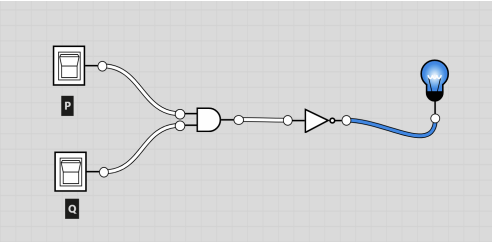
\includegraphics[scale = 1]{circuit.png}
\end{center}

\end{document}